%! Author = Miszka and Tamarka
%! Date = 10.03.2022

% Preamble
\documentclass[11pt]{amsart}

% Packages
\usepackage{float}
\usepackage[T1]{fontenc}
\usepackage{geometry}
\usepackage{parskip}
\usepackage{amsmath}
\usepackage{amsfonts}
\usepackage{amsthm}
\usepackage{amssymb}
\usepackage{titling}
%\usepackage{itemize}
\usepackage{enumerate}
\usepackage{multirow}
\usepackage{graphics}
\usepackage{graphicx}
\usepackage{caption}
\usepackage{array}
\usepackage{xcolor}
\usepackage{subcaption}


\graphicspath{ {./fig/} }


%\setlength{\droptitle}{-2cm}
%\newgeometry{tmargin=1.9cm, bmargin=1.9cm, lmargin=1.7cm, rmargin=1.7cm}

\DeclareMathOperator*{\argmin}{arg\,min}

\newcommand{\tami}[1]{{\textcolor{magenta}{#1}}}
\newcommand{\domi}[1]{{\textcolor{green}{#1}}}

\author{Tamara Frączek, Dominik Mika}
\title{Methods of classification and dimensionality reduction - Report 1}
\date{\today}

% Document
\begin{document}
\maketitle


\section{Introduction}

\subsection*{Statement of the problem}

In this task we have to create a movie recommender system for our users.
\domi{We have users who rated some movies}.
Of course, not every user rated every movie and it is our task to fill those gaps.
So if one user hasn't seen one movie, we want to predict how he would like it.



%some movies and some information about how our users rate our movies.
%Since, of course, not every user rated every movie, we want to predict how they would like the movies from our list.

%We have the data containing information how users rate some movies.
%Our task is to create a recommender system, so having only some data we want to predict all ratings.

For this purpose we build few algorithms using different methods of predicting.
%These methods are described in ...
Of course different methods will give us different results (errors).
Our task is to tune parameters of those methods and try to get the best possible ratings prediction.



\subsection*{Description of methods}

In this problem, we use different methods which are subset of PCA methods. They are often used for dimensionality reduction and matrix factorization.

\subsubsection*{SVD1}

This method gets a $n \times d$ dimensional matrix $Z$ and approximate it by a different matrix $\tilde{Z}$.
Since we want somehow $\tilde{Z}$ to maintain only ''the most important'' information from $Z$, then the rank of $\tilde{Z}$ is to be much smaller than rank of $Z$.
Precisely, we want to find matrix $\tilde{Z}_r$ of rank $r$ ($r < rank(Z)$ and $r$ is a parameter), so that $\|Z - \tilde{Z}_r\|$ is small.

Using SVD decomposition $Z = U \Lambda^{\frac{1}{2}} V^T$ we construct $\tilde{Z}$ as
\[\tilde{Z}_r = U_r \Lambda_r^{\frac{1}{2}}V_r^T,\]
where $\Lambda_r$ contains $r$ biggest eigenvalues of $Z$ and $U_r$, $V_r$ contains only columns corresponding to those eigenvalues.

\subsubsection*{SVD2}

It is an iterative method.
We perform SVD1 on matrix $Z$, then on the result of first SVD1 and so on.
The algorithm can be stopped after a fixed number of iterations or some stop condition can be established.


\subsubsection*{NMF}

Similarly as in SVD1 the method obtain a $n \times d$ dimensional matrix $Z$ and approximate it by $\tilde{Z}$.
This time $\tilde{Z}$ is constructed as $\tilde{Z}_r = W_r H_r $, where $W_r$ and $H_r$ are matrices with non-negative elements ($W_r$ has $r$ columns and $H_r$ has $r$ rows).
Precisely, we look for such $W_r$ and $H_r$ that $\|Z - W_r H_r \|^2$ is the smallest, where $\|A\|^2 = \sum_{i, j} A_{ij}^2$.

\subsubsection*{SGD}

This method, similarly as previous ones want to estimate matrix $Z$ with a product of matrices
$W$ and $H$, but not necessarily obtaining the whole matrix $Z$.

Let's assume that we have only some values of $z_{ij}$ and let call those pairs $(i,j)$ where we know the value of $Z$ as $I$.
We look for
\[\argmin_{W, H} \sum_{(i,j)\in I} (z_{ij} - w_i^T h_j)^2 + \lambda(\|w_i^T\|^2 + \|h_j\|^2),\]
where $h_j$ is $j$-th column of $h$, $w_i^T$ is $i$-th row of $W$ and $\lambda > 0$ is a parameter.
So roughly speaking we look for $W$ and $H$ such that $Z \approx WH$ for elements known in $Z$, but also we want $W$ and $H$ to have quite small values (it gives us the part of sum with parameter $\lambda$).

It is an iterative method and work this way: set some $W$ and $H$,
\begin{enumerate}
    \item sample one pair $(i,j)$ from $I$,
    \item let $\tilde{w}_i^T := w_i^T - \eta \cdot \left(2(z_{ij} - w_i^T h_j) h_j + 2 \lambda w_i^T \right)$ and $\tilde{h}_j := h_j - \eta \cdot \left(2(z_{ij} - w_i^T  h_{j}) w_i^T + 2 \lambda h_j \right)$,
    \item the rests of matrices $W$ and $H$ stay unchanged, so $\tilde{w}_k^T = w_k^T$ for $k \neq i$ and $\tilde{h}_l = h_l$ for $l \neq j$,
    \item take $W = \tilde{W}$ and $H = \tilde{H}$,
\end{enumerate}
and repeat.

$\eta$ is a parameter that tells us how big steps we want to do.
The method stops after a certain number of steps, or it can be given a stop condition.

\section{Implementation}

\subsection*{Description of the data}

Our data contains information 100837 ratings - exactly 610 users rated 9724 movies.
The columns are: \textsf{userId} (integer), \textsf{movieId} (integer) and \textsf{rating} (integer), where \textsf{userId} is a unique user id and \textsf{movieId} is a unique movie id.


We keep this data in two-dimensional matrix of size $n \times d$ where $n$ is the number of users and $d$ is the number of movies.
In element $(i,j)$ we put the rate of the user $i$ of the movie $j$.
If the user $i$ haven't rated the movie $j$ we leave the element empty.


\subsection*{Performing methods}

\tami{??tutaj jakaś intuicja po co dzielić dane??}

So to be able to evaluate the quality of the programs we split our data to two parts: train set and test set.
The train set is used to build the programs.
And the test set is used to evaluate how our programs work.


To give our programs enough information about every user we split the data so that the train set contain 90\% of ratings of each user (and the test set the remaining ones).
\tami{tutaj coś o tym, że będziemy to powtarzać??}

Let call the matrix containing the data from the train set as $\boldsymbol{Z}$ and the matrix containing the data from the test set as $\boldsymbol{T}$.

\tami{??In SVD2 we make a correction -- czy to tu}

\subsection*{Quality of the system}

Assume that our algorithm return a matrix $\boldsymbol{Z}^{'}$.
Then the quality of our programs is computed as \textbf{root-mean square error}
\[\textsf{RMSE} =
\sqrt{\frac{1}{|\mathcal{T}|} \sum_{(u,m) \in \mathcal{T}} \left(\boldsymbol{Z}^{'}[u,m] - \boldsymbol{T}[u,m] \right)^2}\]
where $\mathcal{T}$ contains pairs $(u,m)$ from test set.


\subsection*{Imputing the missing data}

Since three of our methods (SVD1, SVD2 and NMF) are given a full matrix $\boldsymbol{Z}$ then they need the missing data to be imputed before performing.

We decided to impute the data in 5 different ways, we replace missing values with:
\begin{itemize}
    \item 0,
    \item global mean,
    \item column means,
    \item row means,
    \item weighted row and column mean ($\alpha \cdot \text{\textsf{col\_mean}} + (1-\alpha) \cdot \text{\textsf{row\_mean}}$, where $\alpha>0$ is a parameter).
\end{itemize}

We may expect that the closer to reality we impute the missing data, the better results we will obtain.
\tami{tutaj przemyślenia na temat tego czemu niektóre metody działają lepiej i dlaczego}






\section{Parameters tuning}

Before performing our methods and obtaining results we have to set some parameters.

First of all, all the methods need a parameter $r$, which is the rank of matrices in $Z$ decomposition.
SGD needs also learning rate $\eta$ and $\lambda$.
The iteration methods need maximum of possible iterations or a stop condition.

What's more, for all of our methods we want to choose optimal $\alpha$ in the data imputation method with weighted means.



\subsection*{SVD1}
\subsubsection*{Optimizing $r$}
For a start, let's consider only imputation methods that don't need estimation of $\alpha$, so replacing missing values with: 0, global mean, column mean, row mean and weighted row and column mean with $\alpha = \frac{1}{2}$.
%\begin{itemize}
%    \item putting 0 everywhere,
%    \item putting global mean everywhere,
%    \item putting column means,
%    \item putting row means,
%    \item putting weighted row and column mean $\frac{1}{2} \cdot \text{\textsf{col\_mean}} + \frac{1}{2} \cdot \text{\textsf{row\_mean}}$.
%\end{itemize}
%The last method is the weighted method for $\alpha = \frac{1}{2}$.
%These imputation methods will be called \textit{basic} in this report.

For these methods we only need to find optimal $r$ and we will call them \textit{basic}.
So for each of them and for every $r$ from 1 to 100 we perform SVD1.
Below, we present a graph showing results.



\begin{figure}[H]
\centering
\begin{minipage}{.63\textwidth}
  \centering
  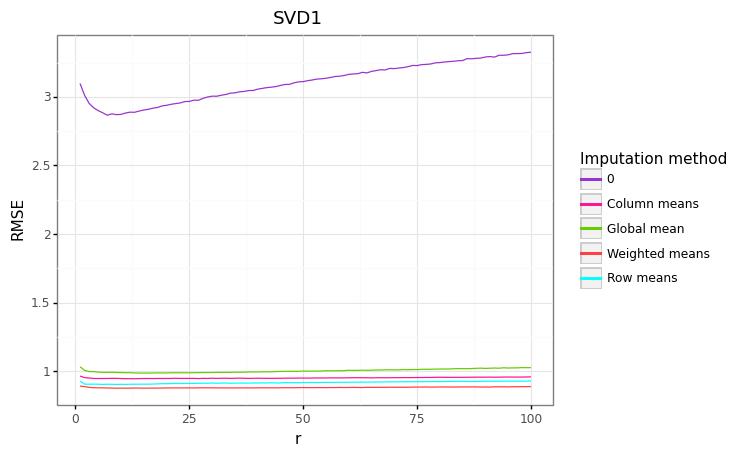
\includegraphics[width=\textwidth]{svd1_1}
%  \captionof{figure}{A figure}
%  \label{fig:test1}
\end{minipage}%
\begin{minipage}{.4\textwidth}
  \centering
  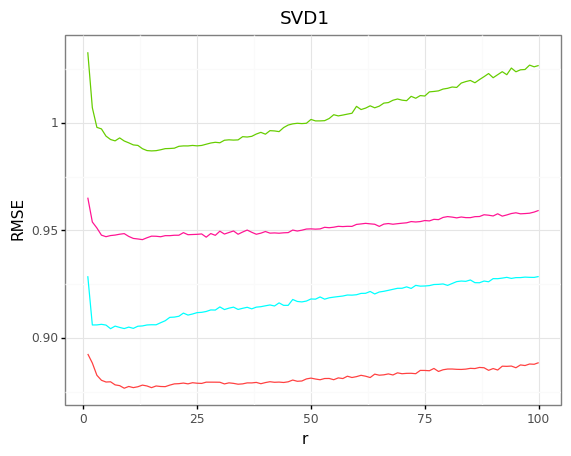
\includegraphics[width=\textwidth]{svd1_2}
%  \captionof{figure}{Another figure}
%  \label{fig:test2}
\end{minipage}
\caption{RMSE of SVD1 for basic imputation methods and $r = 1, \dots, 100$}
\end{figure}

Let's denote that the results in the graph above are computed for the same split of data into train and test set.
%we perform it for only one split of the data into train and test set.
That's why we can compare them.
Also, these results can be much different if we take different split.

Of course we look for the lowest RMSE obtained for each imputation method and the optimal $r$.
So below we present a table containing this information.
\begin{table}[H]
\begin{tabular}{c|ccccc}
& 0 & column means & global mean & weighted means & row means \\
\hline
$r$ & 7 & 13 & 15 & 9 & 6 \\
RMSE & 2.8660 & 0.9458 & 0.9870 & 0.8767 & 0.9043 \\
\end{tabular}
\caption{The lowest RMSE and optimal $r$ for SVD1 with basic imputation methods}
\end{table}
%wnioski, że ma wpływ jak uzupełniamy
%jakieś wnioski, te zera beznadziejne
%że weighted wypadają najlepiej i chcemy to alfa dobrać optymalnie

First of all, from both the graph and the table we can observe that as we expected the choice of the imputation method affects the RMSE.
It can be most clearly seen on an example of data filled with zeros.
For the best $r$ RMSE there is around $2.9$ that is, it is about 3 times larger than for other imputation methods.
Other methods also differ.
The lowest RMSE is obtained for the data filled with weighted data.
But the result for data filled with row means is also quite good.
That's why we may suspect that optimizing $\alpha$ in our weighted imputation method can give even better results.

%wprowadzenie, że dobieramy alfa
%no i ten rysunek wyżej nam pozwala obciąć r
%że robimy minimalizację po dwóch parametrach

\subsubsection*{Optimizing $\alpha$}

To get optimal result we perform optimization with respect to two parameters: $\alpha$ and $r$.
As we can see on the graph above only $r$ between $0$ and $50$ give some reasonable results, so we consider only those (we could use all $r$, but it is time-consuming).
Below, we present graph showing results of optimization.

\begin{figure}[H]
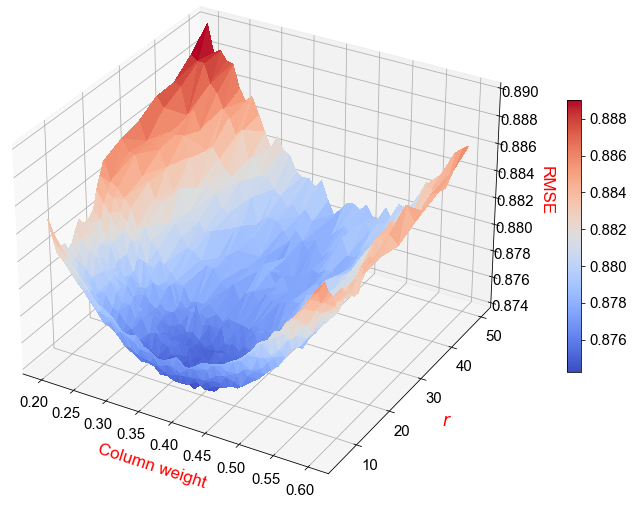
\includegraphics[scale=0.6]{fig/svd1_r_w2}
\label{fig:figure}
\caption{RMSE of SVD1 for weigthed imputation method for different $\alpha$ and $r$}
\end{figure}

Below we present also table with 5 lowest RMSE and pairs $(\alpha, r)$ that gave them.
\begin{table}[H]
\begin{tabular}{cc|c}
 $\alpha$ &  $r$ &     RMSE \\
\hline
       0.39 & 10 & 0.8740 \\
       0.38 & 10 & 0.8742 \\
       0.42 & 10 & 0.8743 \\
       0.36 & 10 & 0.8744 \\
       0.39 & 11 & 0.8745 \\
\end{tabular}
\caption{5 lowest RMSE of SVD1 for weigthed imputation method and ($\alpha$, $r$) that gave them}
\end{table}
Obtained best RMSEs are similar, but they differ in fourth decimal place.
We can observe also that the pair $(0.39, 10)$ seems to be optimal in this case and all other pairs are close to it.


Is this means that we choose the weighted imputation method with $\alpha = 0.39$ and $r=10$ to perform SVD1?
No, because until now, we have considered only one data split into train and test set.
To find the best parameters in our method we have to average optimal $\alpha$ and $r$ over different splits.
So we consider 20 different splits and the results are as follows
\begin{itemize}
    \item mean value of the best $(\alpha, r)$ is $(0.4055, 12.2)$,
    \item median of the best $(\alpha, r)$ is $(0.41, 13)$,
    \item in 15 of 20 cases the best pair is $(0.41, 13)$.
\end{itemize}
\textbf{So $\alpha = 0.41$ and $r = 13$ are the parameters we use in our method SVD1 with weighted means as the imputation method.}







\subsection*{SVD2}
We are going to proceed as in SVD1 case, but before we have to choose some stop condition.

\subsubsection*{Stop condition}
We decided to use the stop condition of following form: if the difference of $Z$ obtained in previous step is enough close to $Z$ obtained in this step we stop the algorithm.
Precisely, we stop algorithm if $\|Z_{n+1} - Z_n\| < \varepsilon$, where $\|\cdot\|$ is the Frobenius norm, $Z_n$ is the matrix obtained in $n$th step and $\varepsilon$ is a parameter to be set.

To find optimal $\epsilon$ we perform an optimization with respect to $r$ and $\epsilon$
on the data filled with weighted means with $\alpha = \frac{1}{2}$.
Below we present the graph with results.

\begin{figure}[H]
    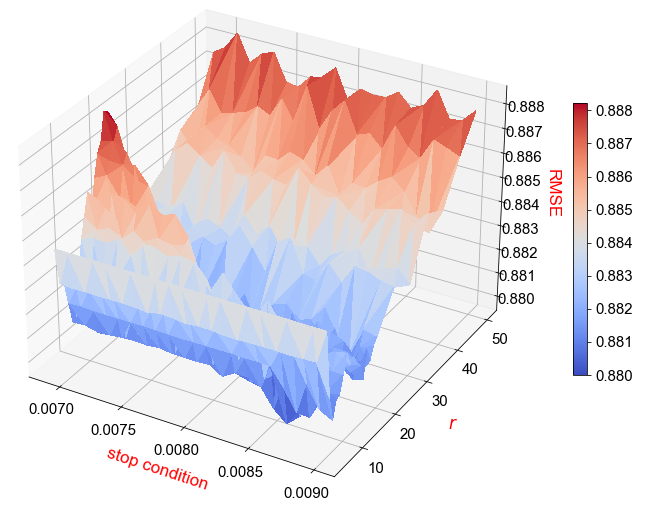
\includegraphics[scale=0.55]{svd2_stop2}
    \caption{RMSE of SVD2 for weigthed imputation method with $\alpha = \frac{1}{2}$ for different $r$ and $\epsilon$}
\end{figure}

\tami{tutaj}


\subsubsection*{Optimizing $r$}
After choosing the stop condition we can proceed exactly as in SVD1 case.
So first we present a graph showing dependence of RMSE on $r$ and on the imputation method for basic imputation methods.
\begin{figure}[H]
\centering
\begin{minipage}{.63\textwidth}
  \centering
  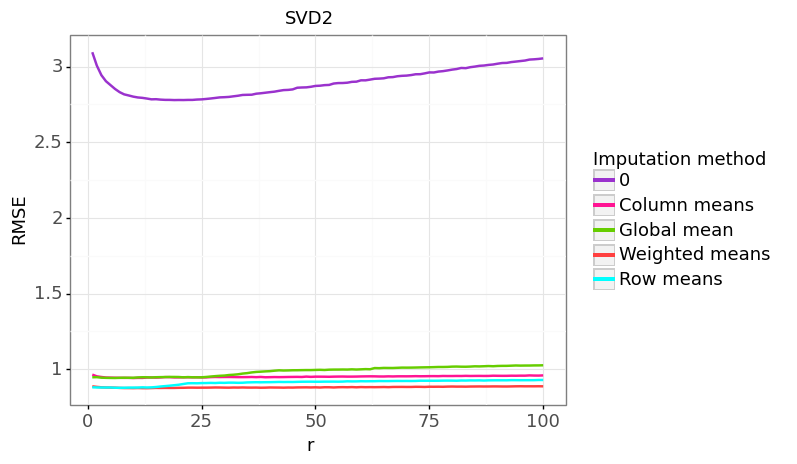
\includegraphics[width=\textwidth]{svd2_1}
%  \captionof{figure}{A figure}
%  \label{fig:test1}
\end{minipage}%
\begin{minipage}{.4\textwidth}
  \centering
  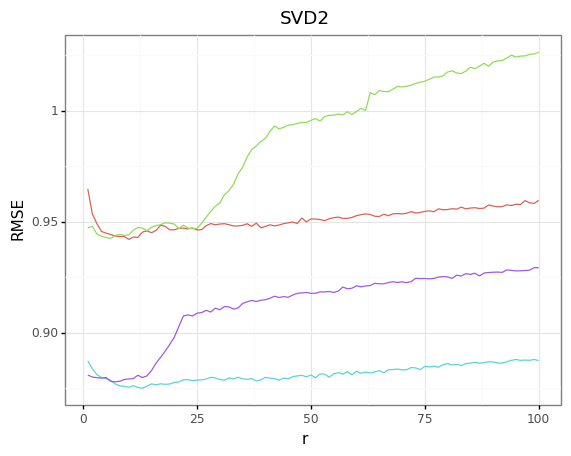
\includegraphics[width=\textwidth]{svd2_2}
%  \captionof{figure}{Another figure}
%  \label{fig:test2}
\end{minipage}
\caption{RMSE of SVD2 for basic imputation methods and $r = 1, \dots, 100$}
\end{figure}

Comparing it with analogous graph for SVD1 we observe bigger ,,jumps'' for imputation methods using global means and row means.
And for these methods best RMSEs are improved.
But after jumps the graph is very similar to the previous one - results and trends are similar.
In case of imputation methods with column means and weighted means doesn't look like the trajectories are changed much.
%\tami{tutaj, że te wykresy są takie bardziej skaczące, ale generalnie trendy są te same}

Now we present a table showing the best $r$ and RMSE for every imputation method.
\begin{table}[H]
\begin{tabular}{c|ccccc}
& 0 & column means & global mean & weighted means & row means \\
\hline
$r$ & 19 & 10 & 6 & 13 & 7 \\
RMSE & 2.7789 & 0.9420 & 0.9425 & 0.8749 & 0.8778 \\
\end{tabular}
\caption{The lowest RMSE and optimal $r$ for SVD2 with basic imputation methods}
\end{table}

Firstly, we can observe that SVD2 improved the results of SVD1.
Every result is smaller, differences are also smaller, but the order which methods are better or worse is the same.

We can observe again that only $r$ between 0 and 50 gives reasonable results.
Though the best $r$ chosen by SVD2 in all cases differ a lot from $r$ chosen by SVD1.

\subsubsection*{Optimizing $\alpha$}
Moving on to the weighted imputation method, we present a graph showing the results of optimization with respect to $\alpha$ and $r$.
\begin{figure}[H]
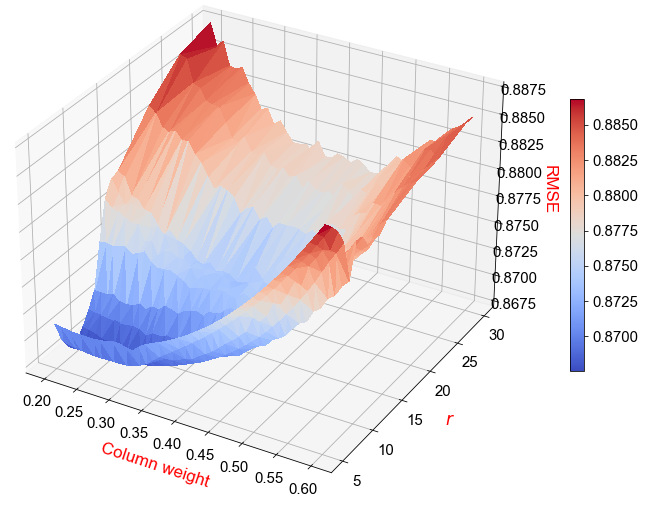
\includegraphics[scale = 0.6]{svd2_r_w2}
\caption{RMSE of SVD2 for weigthed imputation method for different $\alpha$ and $r$}
\end{figure}

The graph differs a lot from the analogous graph for SVD1.
This time the minimum is taken for smaller $\alpha$ and smaller $r$.
\tami{tutaj coś}

To find exact values of minimum let's look at the results in table.

\begin{table}[H]
\begin{tabular}{cc|c}
$\alpha$ &  $r$ &     RMSE \\
\hline
       0.25 &  8 & 0.8674 \\
       0.26 &  8 & 0.8674 \\
       0.24 &  8 & 0.8674 \\
       0.27 &  8 & 0.8674 \\
       0.28 &  8 & 0.8675 \\
\end{tabular}
\caption{5 lowest RMSE of SVD2 for weigthed imputation method and ($\alpha$, $r$) that gave them}
\end{table}
This time method did the best 5 results for the same $r$.
Also in this case, the result are closer.
It is intuitive for iterative method because they usually converge to some specific model and that is why we get clear results.

After repeating this optimization for 20 different splits we get that:
\begin{itemize}
    \item the mean value of the best $(\alpha, r)$ is $(0.259, 8)$,
    \item the median of the best $(\alpha, r)$ is $(0.255, 8)$.
\end{itemize}
\textbf{So $\alpha = 0.26$ and $r=8$ are parameters we use in our SVD2 with weighted means as the imputation method.}

\subsection*{NMF}
In this case since we have only $r$ and $\alpha$ to find, we proceed in exactly the same way as in the case of SVD.

\subsubsection*{Optimizing $r$}
So firstly we present a graph showing dependence of RMSE on $r$ and on the imputation method for basic imputation methods.

\begin{figure}[H]
\centering
\begin{minipage}{.63\textwidth}
  \centering
  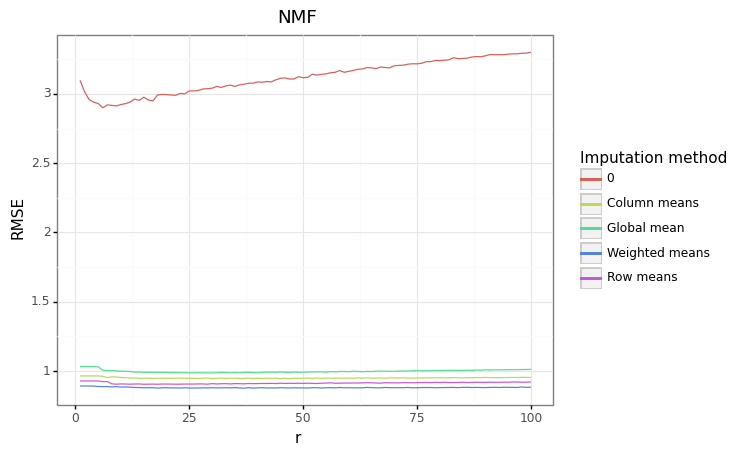
\includegraphics[width=\textwidth]{nmf_1}
%  \captionof{figure}{A figure}
%  \label{fig:test1}
\end{minipage}%
\begin{minipage}{.4\textwidth}
  \centering
  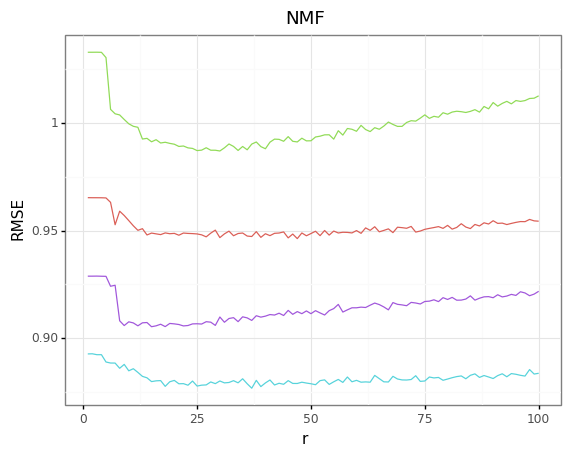
\includegraphics[width=\textwidth]{nmf_2}
%  \captionof{figure}{Another figure}
%  \label{fig:test2}
\end{minipage}
\caption{RMSE of NMF for basic imputation methods and $r = 1, \dots, 100$}
\end{figure}

Comparing this graph to the graph for SVDs we observe that the previous graphs where smoother.
This time trajectories oscillate a lot, which means that for similar $r$ it gives quite different RMSE.
So this method seem more unstable than the previous ones.

What's more, here it is not so obvious where to look for optimal $r$.
For instance for imputation method with weighted means RMSE don't grow much with greater $r$.

Nevertheless, the order of methods (so which one is the best and so on) is the same.

Below we also present a table with the lowest RMSE for every imputation method and the parameter $r$ that gave it.

\begin{table}[H]
\begin{tabular}{c|ccccc}
& 0 & column means & global mean & weighted means & row means \\
\hline
$r$ & 6 & 47 & 30 & 37 & 15\\
RMSE & 2.8997 & 0.9462 & 0.9870 & 0.8766 & 0.9053 \\
\end{tabular}
\caption{The lowest RMSE and optimal $r$ for NMF with basic imputation methods}
\end{table}

As we can see the parameters $r$ are in general bigger than in previous cases.
The RMSEs are very similar to those obtained using SVD1.

\subsubsection*{Optimizing $\alpha$}
Now we perform the optimization with respect to $\alpha$ and $r$ and present a graph showing the results.

\begin{figure}[H]
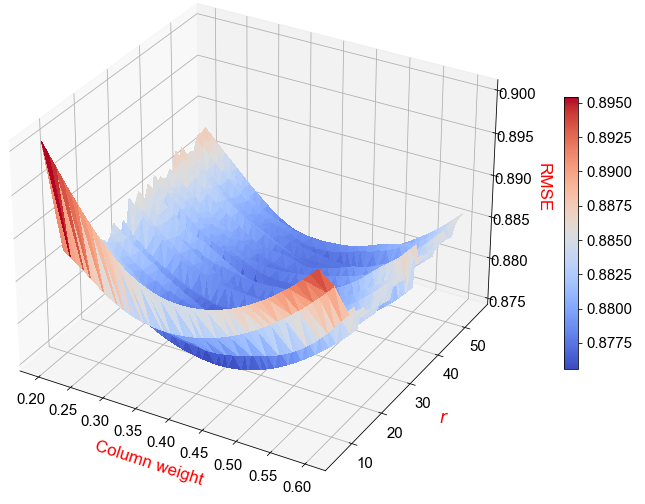
\includegraphics[scale = 0.6]{nmf_r_w2}
\caption{RMSE of NMF for weigthed imputation method for different $\alpha$ and $r$}
\end{figure}

Comparing this graph to previuos analogous graphs this one is completely different.
RMSE in here doen't grow much with growth of $r$.
Similarly as in previuos graph for NMF, this graph oscillates a lot looking at the axis of $r$.

To find where is the minimum of RMSE taken we have to look at the results in table.

\begin{table}[H]
\begin{tabular}{cc|c}
$\alpha$ &  $r$ &     RMSE \\
\hline
       0.40 & 37 & 0.8748 \\
       0.41 & 37 & 0.8748 \\
       0.39 & 18 & 0.8748 \\
       0.39 & 37 & 0.8748 \\
       0.40 & 18 & 0.8748 \\
\end{tabular}
\caption{5 lowest RMSE of NMF for weigthed imputation method and ($\alpha$, $r$) that gave them}
\end{table}

\tami{ważne wnioski, że te r są takie różne, a wyniki bardzo bliskie}

After repeating this optimization for 20 different splits we get that:
\begin{itemize}
    \item the mean value of the best $(\alpha, r)$ is $(0.393, 32.25)$,
    \item the median of the best $(\alpha, r)$ is $(0.39, 37)$,
    \item 15 times the best $r$ is 37 and 5 times the best $r$ is 18.
\end{itemize}
\textbf{So $\alpha = 0.39$ and $r=37$ are parameters we use in our NMF with weighted means as the imputation method.}




\subsection*{SGD}
$5\cdot 10^{-10}$, faktyczna- $10^{-11}$(norma $L_1$)
$r = 5$
$\lambda = 0.01$
$\eta = 0.007$

%\begin{figure}[H]
%\centering
%\begin{minipage}{.5\textwidth}
%  \centering
%  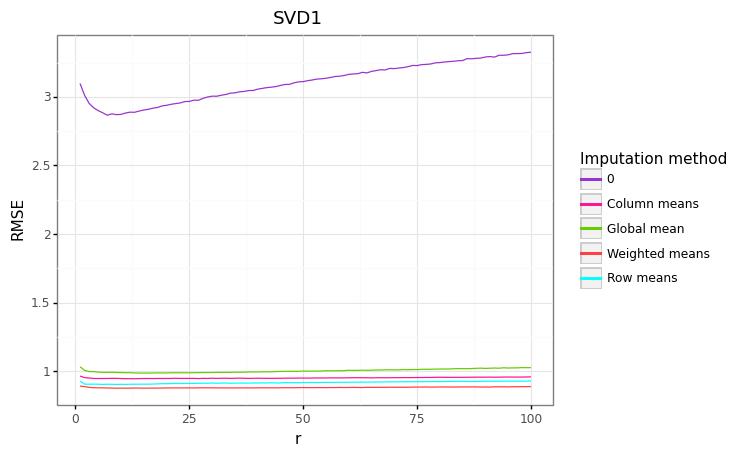
\includegraphics[scale=0.43]{svd1_1}
%%  \captionof{figure}{A figure}
%%  \label{fig:test1}
%\end{minipage}%
%\begin{minipage}{.5\textwidth}
%  \centering
%  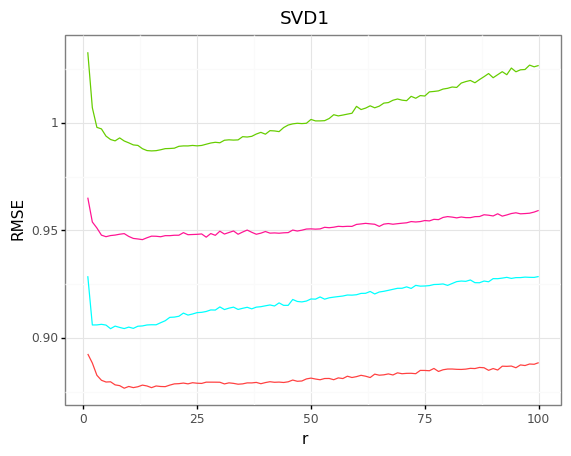
\includegraphics[scale=0.43]{svd1_2}
%%  \captionof{figure}{Another figure}
%%  \label{fig:test2}
%\end{minipage}
%\end{figure}



\section{}

\section{Results}

Since in columns we keep indexes of movies, it means that our filled data take a bit more information from user ratings mean than from the movie ratings mean.
That is probably logical \tami{...}

\end{document}